\subsection{The kernel density estimator}
The main tool for density estimation would be the GMM method, but since this method can be computationally heavy with larger data sets, and sensitive to the initial conditions, a deterministic approximation is used instead which is called the kernel density estimator (KDE). The approximations from GMM are; weights are set as equal, $K$ is set to $N$ meaning $\mathbf{\mu}_k$ is set to the $\mathbf{x}_i$ and the covariance matrix is diagonalized as $\lambda^2 \mathbf{I}$. This leads to the probability function seen in eq. \eqref{eq:KDE}.
\begin{equation} \label{eq:KDE}
    p_{\lambda}(\mathbf{x}) = \frac{1}{N} \sum^N_{i=1} \mathcal{N}(\mathbf{x} \mid \mathbf{x}_i, \lambda^2 \mathbf{I} )
\end{equation}
where only $\lambda$ must be evaluated which gives a great performance enhancement. The $\lambda$ is called the kernel width and controls the width of the probability curve fitted. This width is found through cross-validation with the goal of maximizing the log of the likelihood, similar to when evaluating the parameters of GMM, using the expectation maximization algorithm, outlined in the section 17.2 of the course notes \cite{coursenotes}.

The density estimation is then based on how probable an observation is, by the probability function \eqref{eq:KDE}.

\begin{wrapfigure}{r}{0.5\textwidth}
    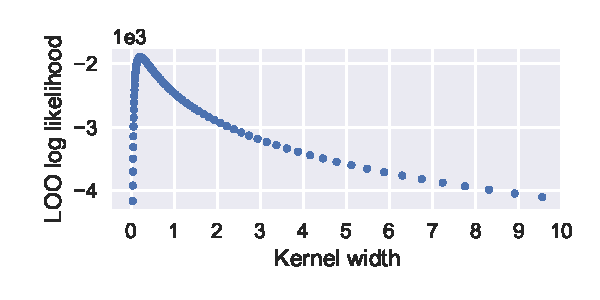
\includegraphics[width=\linewidth]{fig/KDE_LOO.pdf}
    \caption{Log of the likelihood by leave-one-out cross validation for different kernel widths.}
    \label{fig:KDE_LOO}
\end{wrapfigure}

For the glass data set, we can calculate the kernel width using leave-one-out cross validation, resulting in the probability function which predicts the new observation with the highest accuracy. The log of the likelihood for each kernel width is seen in figure \ref{fig:KDE_LOO}.

The optimal width is found to be $\lambda = 0.211$.

Once this is found, we can calculate the density score using eq.\eqref{eq:KDE} at each observation. The lowest 20 density scores are shown in figure \ref{fig:KDE_DensityScore}. The orders of magnitude between the lowest 20 observations density scores, suggest that the data set contains observations with highly improbable attribute values. 

The interval of density scores is $[7.4 \cdot 10^{-60}, 2.87 \cdot 10^{-2}]$, and from the density score distribution in figure \ref{fig:KDE_DensityDistribution}, it is clear that the majority of the observations are found in low density areas.

\begin{multicols}{2}
\begin{figure}[H]
    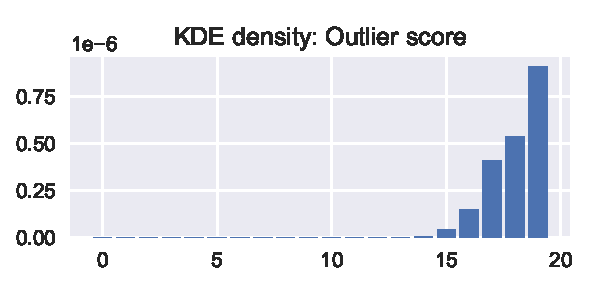
\includegraphics[width=\linewidth]{fig/KDE_densitybarplot_lowest20.pdf}
    \caption{20 lowest density scores using eq. \eqref{eq:KDE}.}
    \label{fig:KDE_DensityScore}
\end{figure}

\begin{figure}[H]
    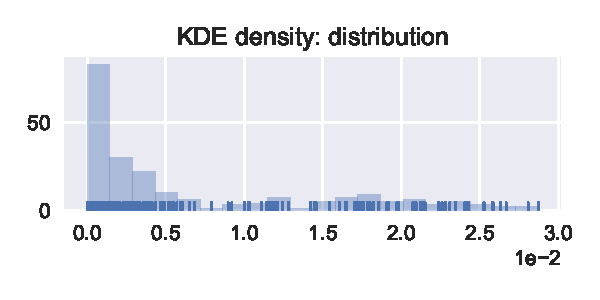
\includegraphics[width=\linewidth]{fig/KDE_densitydistribution.pdf}
    \caption{Density score distribution for the entire data set.}
    \label{fig:KDE_DensityDistribution}
\end{figure}
\end{multicols}

The KDE method does not differentiate between clusters of high and low densities, as the kernel width is the same across the data set, which result in some observations having such low density scores. 